\documentclass{beamer}
\mode<presentation>
\usepackage{amsmath,amssymb,mathtools}
\usepackage{textcomp}
\usepackage{gensymb}
\usepackage{adjustbox}
\usepackage{subcaption}
\usepackage{enumitem}
\usepackage{multicol}
\usepackage{listings}
\usepackage{url}
\usepackage{graphicx} % <-- needed for images
\def\UrlBreaks{\do\/\do-}

\usetheme{Boadilla}
\usecolortheme{lily}
\setbeamertemplate{footline}{
  \leavevmode%
  \hbox{%
  \begin{beamercolorbox}[wd=\paperwidth,ht=2ex,dp=1ex,right]{author in head/foot}%
    \insertframenumber{} / \inserttotalframenumber\hspace*{2ex}
  \end{beamercolorbox}}%
  \vskip0pt%
}
\setbeamertemplate{navigation symbols}{}

\lstset{
  frame=single,
  breaklines=true,
  columns=fullflexible,
  basicstyle=\ttfamily\tiny   % tiny font so code fits
}

\numberwithin{equation}{section}

% ---- your macros ----
\providecommand{\nCr}[2]{\,^{#1}C_{#2}}
\providecommand{\nPr}[2]{\,^{#1}P_{#2}}
\providecommand{\mbf}{\mathbf}
\providecommand{\pr}[1]{\ensuremath{\Pr\left(#1\right)}}
\providecommand{\qfunc}[1]{\ensuremath{Q\left(#1\right)}}
\providecommand{\sbrak}[1]{\ensuremath{{}\left[#1\right]}}
\providecommand{\lsbrak}[1]{\ensuremath{{}\left[#1\right.}}
\providecommand{\rsbrak}[1]{\ensuremath{\left.#1\right]}}
\providecommand{\brak}[1]{\ensuremath{\left(#1\right)}}
\providecommand{\lbrak}[1]{\ensuremath{\left(#1\right.}}
\providecommand{\rbrak}[1]{\ensuremath{\left.#1\right)}}
\providecommand{\cbrak}[1]{\ensuremath{\left\{#1\right\}}}
\providecommand{\lcbrak}[1]{\ensuremath{\left\{#1\right.}}
\providecommand{\rcbrak}[1]{\ensuremath{\left.#1\right\}}}
\theoremstyle{remark}
\newtheorem{rem}{Remark}
\newcommand{\sgn}{\mathop{\mathrm{sgn}}}
\providecommand{\abs}[1]{\left\vert#1\right\vert}
\providecommand{\res}[1]{\Res\displaylimits_{#1}}
\providecommand{\norm}[1]{\lVert#1\rVert}
\providecommand{\mtx}[1]{\mathbf{#1}}
\providecommand{\mean}[1]{E\left[ #1 \right]}
\providecommand{\fourier}{\overset{\mathcal{F}}{ \rightleftharpoons}}
\providecommand{\system}{\overset{\mathcal{H}}{ \longleftrightarrow}}
\providecommand{\dec}[2]{\ensuremath{\overset{#1}{\underset{#2}{\gtrless}}}}
\newcommand{\myvec}[1]{\ensuremath{\begin{pmatrix}#1\end{pmatrix}}}
\let\vec\mathbf

\title{Matgeo Presentation - Problem 12.492}
\author{ee25btech11063 - Vejith}

\begin{document}


\frame{\titlepage}
\begin{frame}{Question}
Direction cosines of the vector $3\vec{\hat{i}} + -2\vec{\hat{j}} + 6\vec{\hat{k}}$ are
\begin{enumerate}[label=\alph*)]
    \begin{multicols}{2}
        \item \sbrak{3/7,-2/7,6/7}
        \item \sbrak{-3/7,2/7,-6/7}
       \item \sbrak{-7/3,7/2,-7/6}
        \item \sbrak{7/3,-7/2,7/6}
    \end{multicols}
\end{enumerate}
\end{frame}

\begin{frame}{Solution}
    let 
\begin{align}
    \Vec{r} = \myvec{3\\-2\\6}\\
    \norm{\vec{r}}=\sqrt{9 +4 +36}\\
\implies \norm{\vec{r}}=7
\end{align}
The unit  vector in the direction of $\vec{r}$  is
\begin{align}
    \frac{\vec{r}}{\norm{\vec{r}}} &= \frac{1}{7}\myvec{3\\-2\\6} = \myvec{\frac{3}{7}\\\frac{-2}{7}\\\frac{6}{7}}
    \end{align}
\end{frame}

\begin{frame}{Plot}
     \begin{figure}[h!]
   \centering
   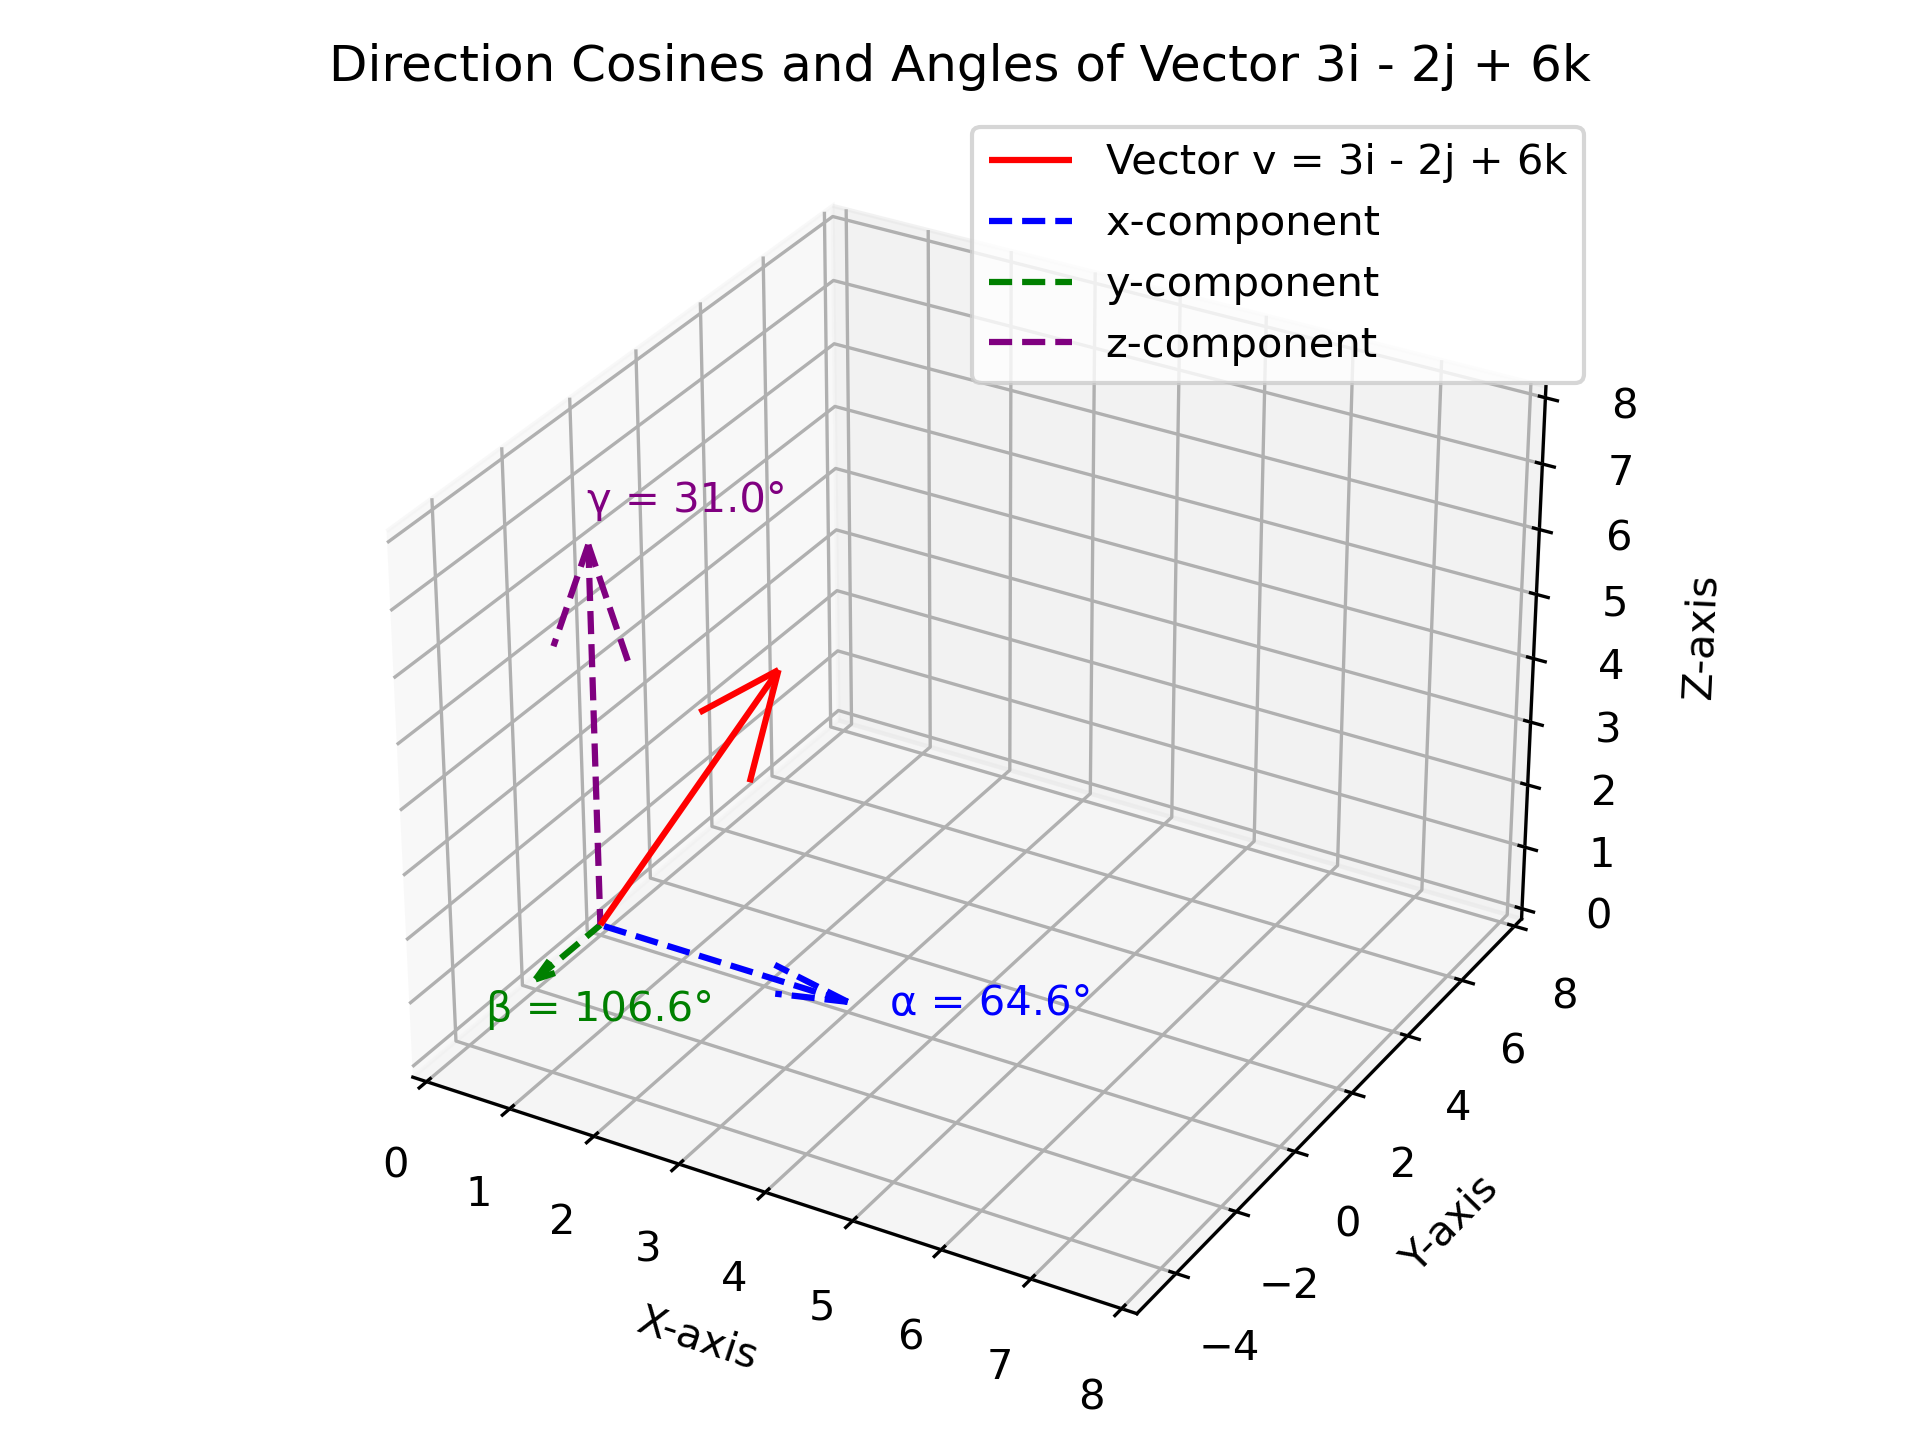
\includegraphics[width=0.9\columnwidth]{figs/01.png}
   \caption{}
   \label{}
\end{figure}
\end{frame}

% --------- CODE APPENDIX ---------
\section*{Appendix: Code}

% C program
\begin{frame}[fragile]{C Code: dc.c}
\begin{lstlisting}[language=C]
#include <stdio.h>
#include <math.h>

int main() {
    // Vector components
    int x = 3, y = -2, z = 6;
    double magnitude, l, m, n;

    // Calculate magnitude
    magnitude = sqrt(x*x + y*y + z*z);

    // Direction cosines
    l = x / magnitude;
    m = y / magnitude;
    n = z / magnitude;

    // Open file for writing
    FILE *fp = fopen("dc.dat", "w");
    if (fp == NULL) {
        printf("Error opening file!\n");
        return 1;
    }

    fprintf(fp, "Direction cosines of vector (3, -2, 6):\n");
    fprintf(fp, "l = %.4f\n", l);
    fprintf(fp, "m = %.4f\n", m);
    fprintf(fp, "n = %.4f\n", n);

    fclose(fp);
    printf("Output written to dc.dat successfully.\n");

    return 0;
}
\end{lstlisting}
\end{frame}

% Python plotting
\begin{frame}[fragile]{Python: plot.py}
\begin{lstlisting}[language=Python]
import numpy as np
import matplotlib.pyplot as plt
from mpl_toolkits.mplot3d import Axes3D

# Vector components
a, b, c = 3, -2, 6
v = np.array([a, b, c])

# Magnitude of vector
magnitude = np.linalg.norm(v)

# Direction cosines
cos_alpha = a / magnitude
cos_beta  = b / magnitude
cos_gamma = c / magnitude

# Direction angles in degrees
alpha = np.degrees(np.arccos(cos_alpha))
beta  = np.degrees(np.arccos(cos_beta))
gamma = np.degrees(np.arccos(cos_gamma))

# Print direction cosines and angles
print(f"Direction cosines: ({cos_alpha:.2f}, {cos_beta:.2f}, {cos_gamma:.2f})")
print(f"Direction angles (degrees): α = {alpha:.2f}°, β = {beta:.2f}°, γ = {gamma:.2f}°")

# 3D Plot
fig = plt.figure()
ax = fig.add_subplot(111, projection='3d')

# Plot the vector
ax.quiver(0, 0, 0, a, b, c, color='r', label='Vector v = 3i - 2j + 6k')
  \end{lstlisting}
\end{frame}

\begin{frame}[fragile]{Python: plot.py}
\begin{lstlisting}[language=Python]
# Plot projections on axes
ax.quiver(0, 0, 0, a, 0, 0, color='blue', linestyle='dashed', label='x-component')
ax.quiver(0, 0, 0, 0, b, 0, color='green', linestyle='dashed', label='y-component')
ax.quiver(0, 0, 0, 0, 0, c, color='purple', linestyle='dashed', label='z-component')

# Annotate angles with adjusted positions to avoid overlap
ax.text(a + 0.5, 0, 0, f'α = {alpha:.1f}°', color='blue', fontsize=10)
ax.text(0, b - 1.5, 0, f'β = {beta:.1f}°', color='green', fontsize=10)
ax.text(0, 0, c + 0.5, f'γ = {gamma:.1f}°', color='purple', fontsize=10)

# Axes limits
max_val = max(abs(a), abs(b), abs(c)) + 2
ax.set_xlim([0, max_val])
ax.set_ylim([min(0, b) - 3, max_val])
ax.set_zlim([0, max_val])

# Labels
ax.set_xlabel('X-axis')
ax.set_ylabel('Y-axis')
ax.set_zlabel('Z-axis')
ax.set_title('Direction Cosines and Angles of Vector 3i - 2j + 6k')
ax.legend()

plt.tight_layout()

# Save the figure
plt.savefig('direction_cosines_vector.png', dpi=300)
print("Plot saved as 'direction_cosines_vector.png'")

plt.show()

    \end{lstlisting}
\end{frame}
\end{document}
